\section{Context}

% TODO: i think we should merge the two first slides together (Context and Existing Tools)
% And put the images grid in the "My Research Project" slide

\begin{frame}
    \begin{columns}
        \column{0.5\textwidth}
        \customframetitle{Context - Overall Project}
        
        \vspace{1em}
        
        \begin{itemize}
            \itemsep1em
            \item Professional Bouldering.
            \item \textbf{Goal:} improve climbers' performance.
            \item Tools to help are being developed.
            \item To understand climbing behavior.
        \end{itemize}

        \column{0.45\textwidth}
        \begin{figure}[!t]
            \centering
            \fbox{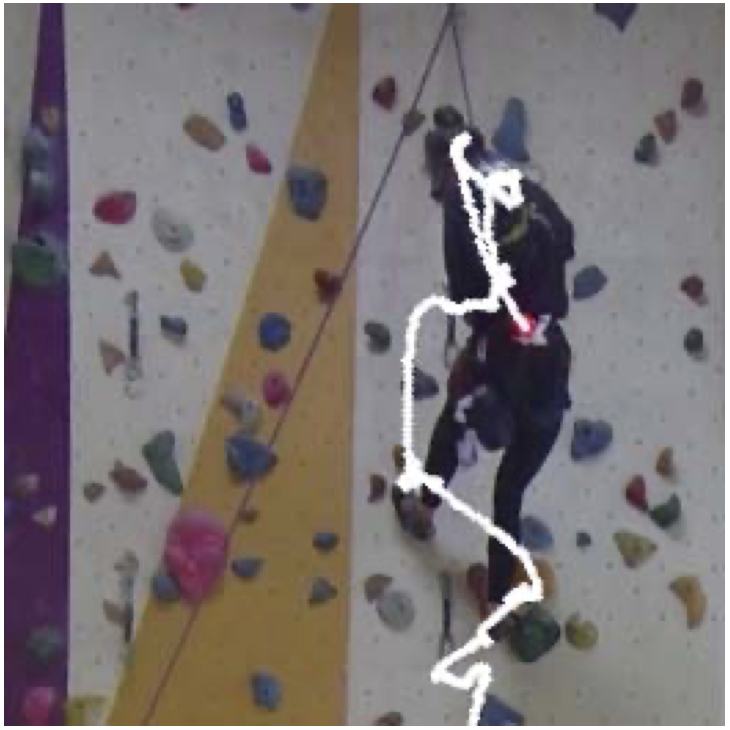
\includegraphics[width=0.8\textwidth]{../../assets/images/climber-path-tracking.png}} 
            \caption{Grip Detection Model.}
            \label{figure:path-tracking}
            \cite{boulanger2025automatic}
        \end{figure}
    \end{columns}

    % Climb Tracking: https://beta-angel.com/wp-content/uploads/2019/03/speed-wall-phases4-1.png
    % Grip Detection: https://www.12climb.com/wp-content/uploads/2019/07/Group-77.jpg
\end{frame}

\begin{frame}
    \begin{columns}
        \column{0.5\textwidth}
        \customframetitle{Context - My Research Project}
        
        \vspace{1em}

        Distinct between different phases of bouldering.
        
        \vspace{1em}

        \begin{itemize}
            \itemsep1em
            \item Given a 4mins bouldering video.
            \item Segment the video in time.
            \item Detect the climber's Activity.
        \end{itemize}

        \column{0.5\textwidth}
        \begin{figure}[!t]
            \centering
            \begin{tabular}{@{}c@{\hspace{4pt}}c@{}}
                \fbox{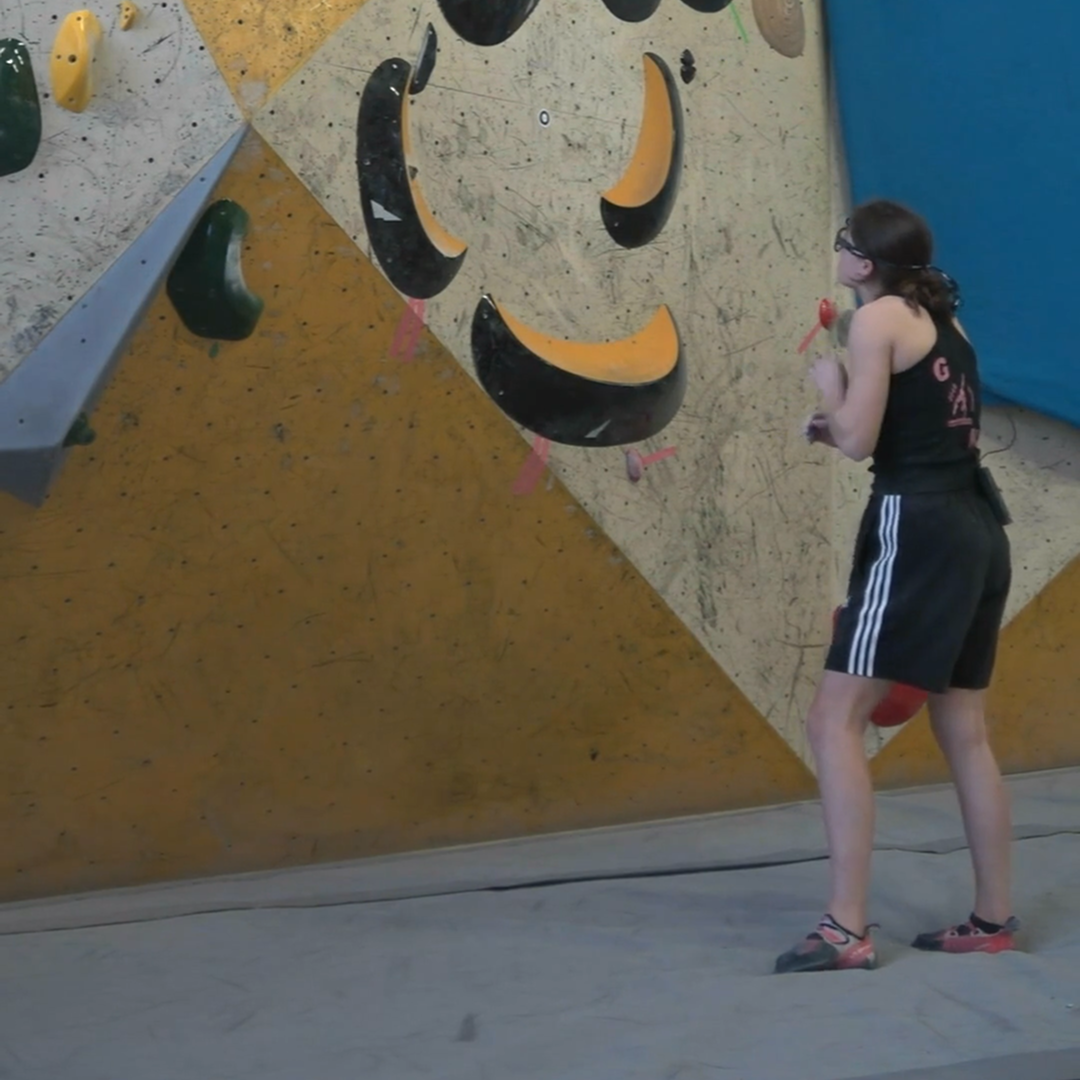
\includegraphics[width=0.4\textwidth]{../../assets/images/observing.2.square.png}} &
                \fbox{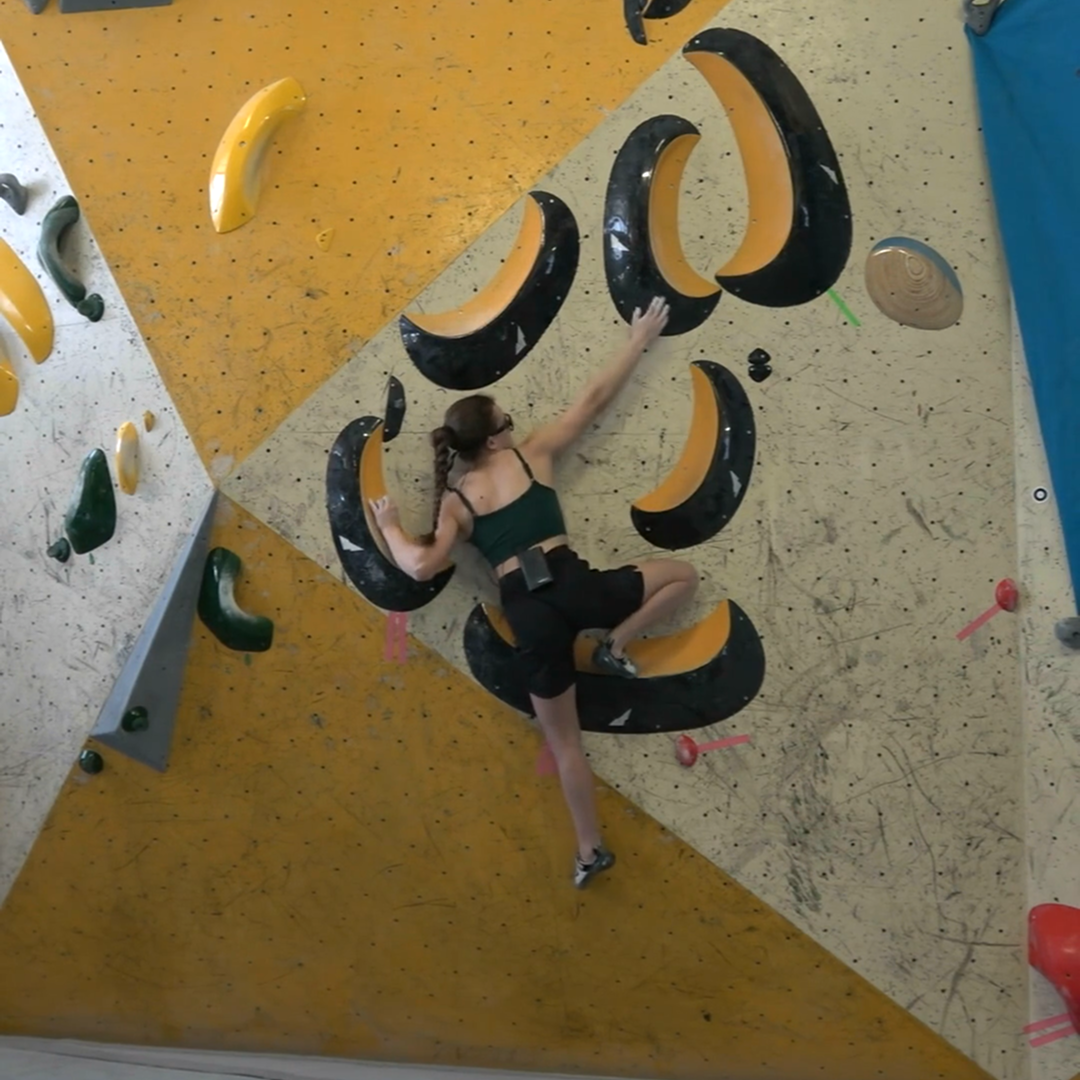
\includegraphics[width=0.4\textwidth]{../../assets/images/climbing.1.square.png}} \\
                {\scriptsize Reading.} & {\scriptsize Climbing.} \\

                \fbox{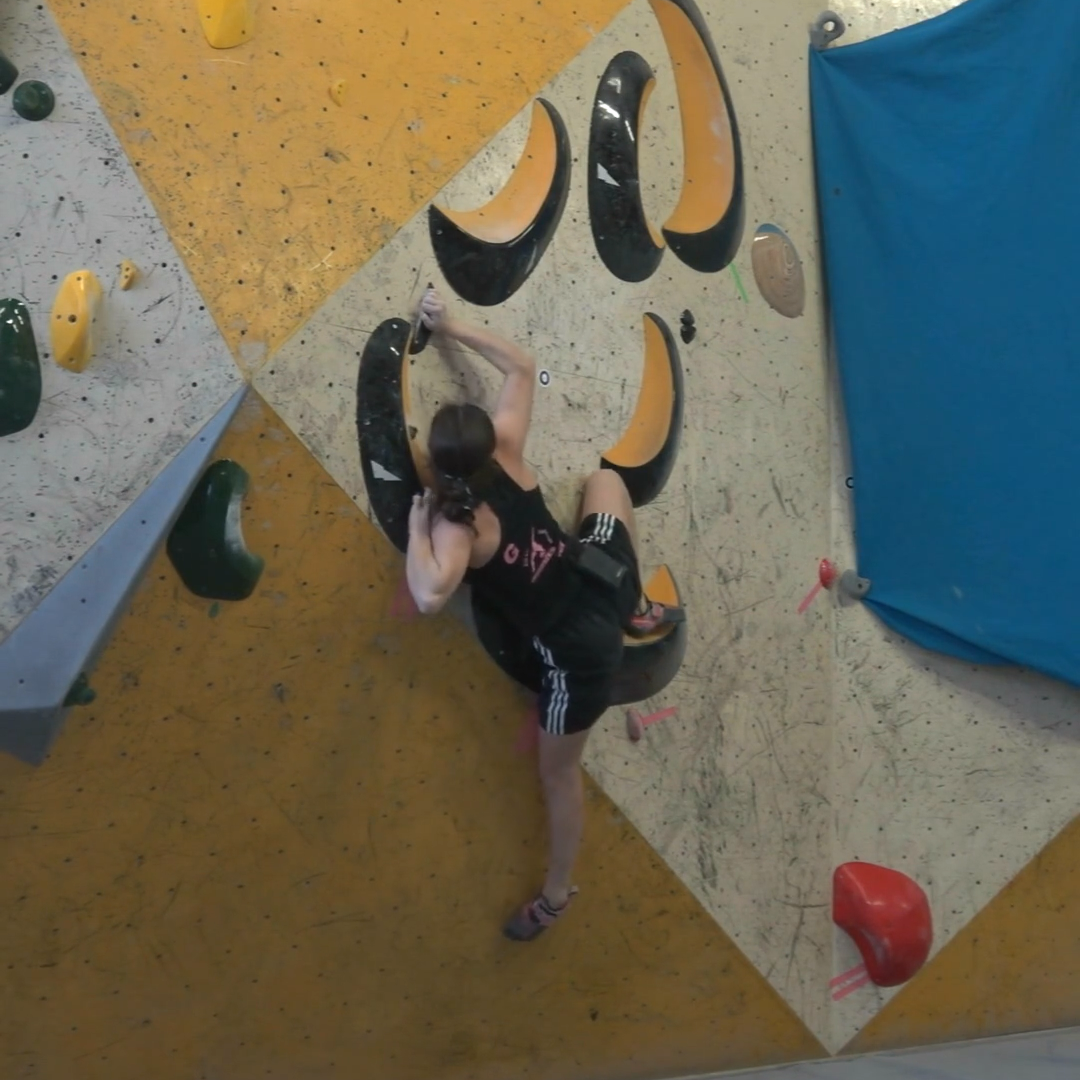
\includegraphics[width=0.4\textwidth]{../../assets/images/climbing.2.square.png}} &
                \fbox{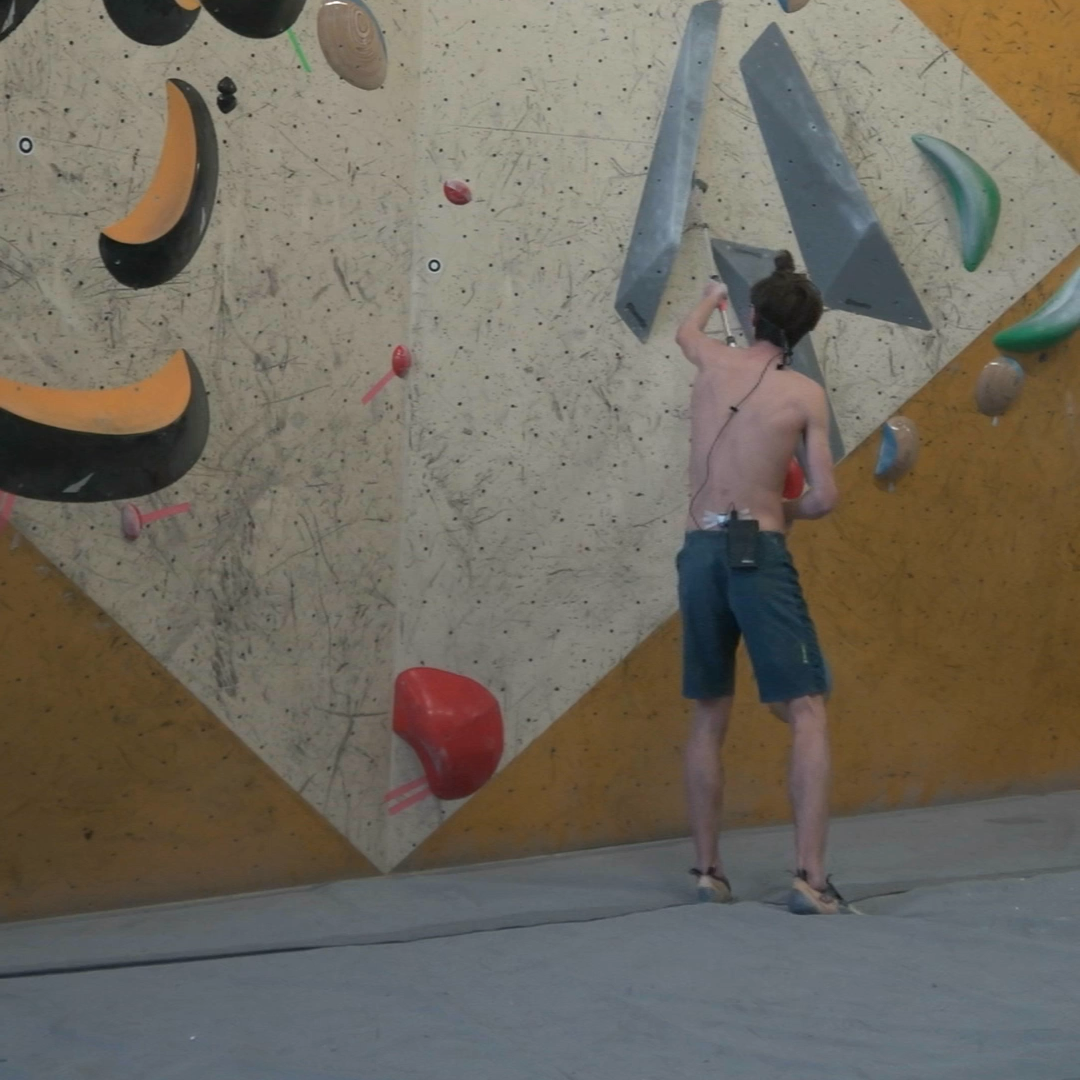
\includegraphics[width=0.4\textwidth]{../../assets/images/brushing.3.square.png}} \\
                {\scriptsize Climbing.} & {\scriptsize Brushing.}
            \end{tabular}
            % \caption{Different phases of bouldering.}
            \label{figure:phases-of-bouldering}
        \end{figure}
    \end{columns}
\end{frame}